%
% Slides for my bachelor's thesis defense.
%
% 1st dry-run: 11:30 minutes
%   Remember to say what a k-mer is; maybe have separate slide about K-Clust
%   or at least show the intersection criterion.
%
% 2nd dry-run: 12:40 minutes
%   Give more introduction, not just directly into the problem of partitioning
%   sequencs.
%
\documentclass{beamer}

\usepackage[utf8]{inputenc}
\usepackage{graphicx}
\usepackage{xcolor}
\usepackage{url}
\usepackage{amsmath, amsthm}
\usepackage{mathtools}
\usepackage{stmaryrd}
\usepackage{adjustbox}

% algorithms
\usepackage{algorithm}            % algorithm float environment
\usepackage[noend]{algpseudocode} % from algorithmicx

% \abs{} command
\DeclarePairedDelimiter\abs{\lvert}{\rvert}
\makeatletter
\let\oldabs\abs
\def\abs{\@ifstar{\oldabs}{\oldabs*}}

\newtheorem{mydef}{Definition}

\usetheme{Copenhagen}
\usecolortheme{default}
\beamertemplatenavigationsymbolsempty

\title{Efficient DNA/RNA sequence clustering}
\subtitle{Using $k$-mers as an approximation for sequence similarity}
\author{Anders Kiel Hovgaard}
\institute{Department of Computer Science, University of Copenhagen}
\date{June 18, 2015}

\begin{document}

% {{{ Title page  -------------------------------------------------------------
\frame{\titlepage}
% }}}

% {{{ Introduction ------------------------------------------------------------
\section{Introduction}

\begin{frame}
  \frametitle{Introduction}
  \framesubtitle{Defining the clustering problem to be solved}

  Partitioning of sequences into a minimal number of clusters based on a
  measure of similarity between sequences.

  \begin{figure}
    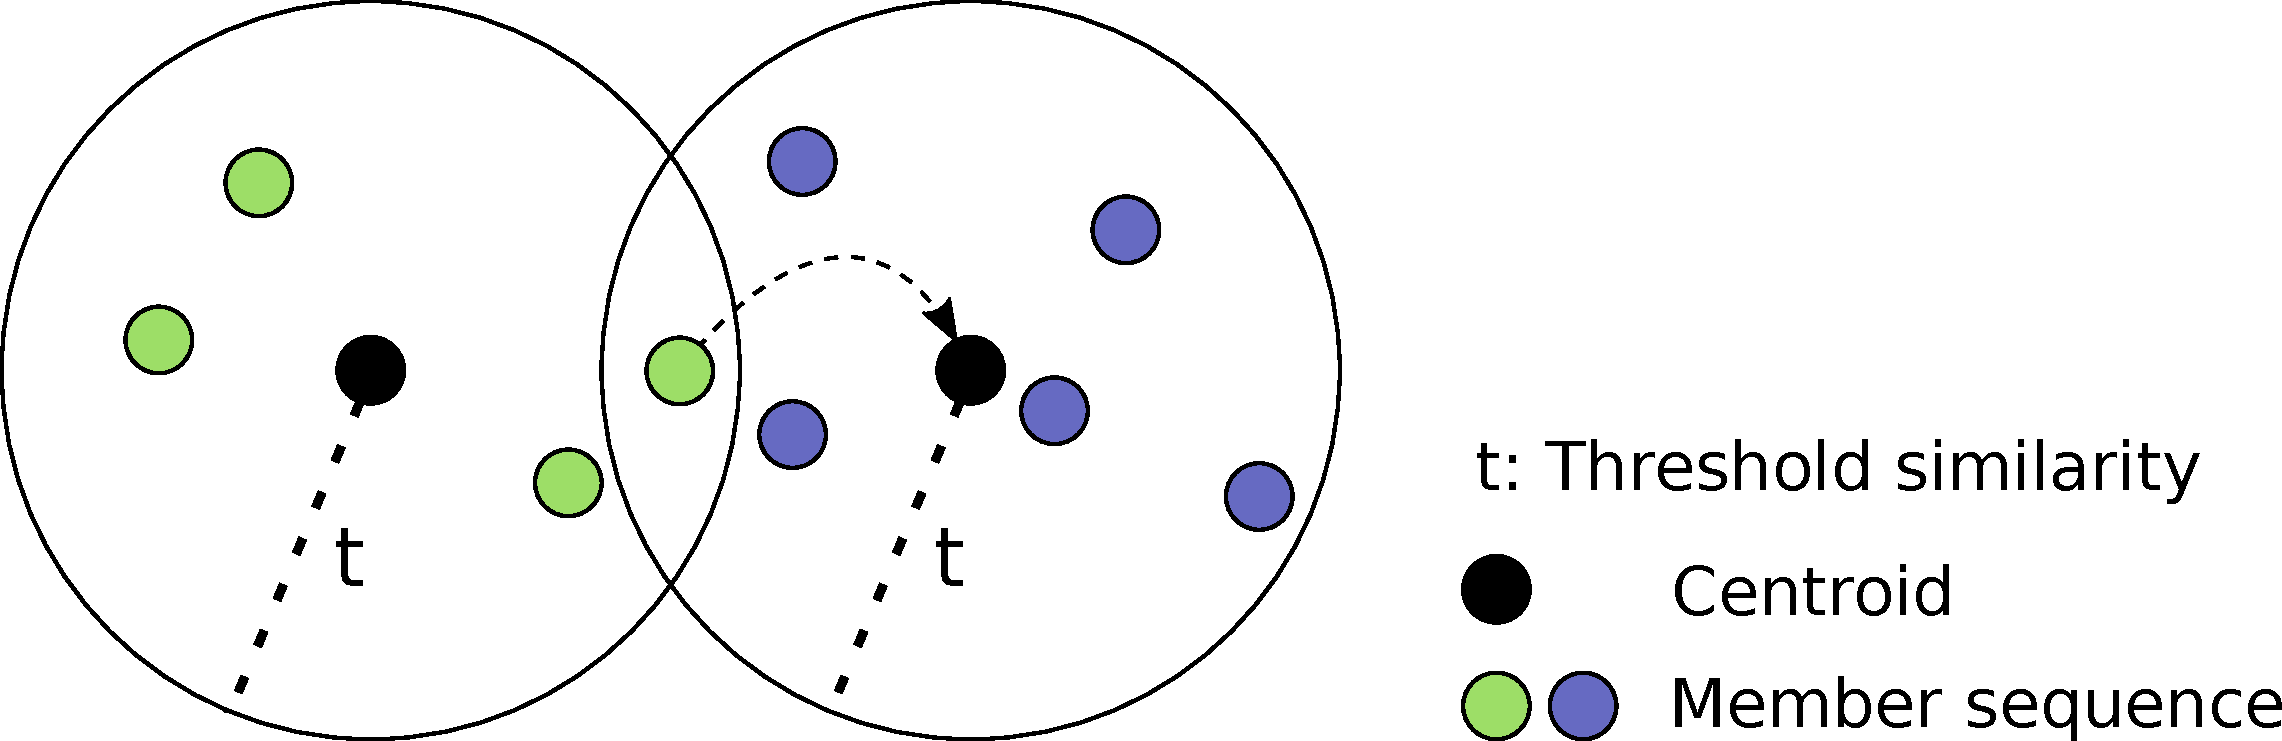
\includegraphics[width=0.7\textwidth]{graphics/centroid-clustering.pdf}
  \end{figure}

  \begin{itemize}
    \item How to measure similarity/distance between sequences?
    \item How to cluster sequences based on such a measure?
  \end{itemize}
\end{frame}
% }}}

% {{{ Distance metrics --------------------------------------------------------
\section{Distance metrics}
\subsection{Various distance metrics}

\begin{frame}{Distance metrics}
  There are various distance metrics:

  \begin{itemize}
    \item edit distance, Levenshtein
    \item sequence alignment
    \item feature based distance, $k$-mer counting
      \begin{itemize}
        \item \textsc{K-Dist} uses a kind of $k$-mer counting
      \end{itemize}
  \end{itemize}
\end{frame}

\subsection{The simple $d2$ distance}

\begin{frame}{The simple $d2$ distance}
  \begin{align*}
    S_1 &= ACTACAC \\
    S_2 &= ACAGAT
  \end{align*}
  \vspace{-1.5em}
  \begin{itemize}
    \item Fill vectors with $k$-mer counts
  \end{itemize}
  \begin{table}[h]
    \centering
    \scalebox{0.75}{
    \begin{tabular}{c | c c c c c c c c c c c c c c c c}
            & AC & AG & AT & CA & CT & GA & TA \\
      \hline
      $S_1$ & 3  &    &    & 1  & 1  &    & 1  \\
      \hline
      $S_2$ & 1  & 1  & 1  & 1  &    & 1  &    \\
    \end{tabular}}
  \end{table}

  \begin{itemize}
    \item Calculate the Euclidean distance
  \end{itemize}
  \begin{align*}
    d2_2(S_1, S_2)
      &= \sqrt{(3-1)^2 - 1^2 - 1^2 + (1-1)^2 + 1^2 - 1^2 + 1^2} \\
      &= \sqrt{9} = 3
  \end{align*}
\end{frame}

\subsection{The \textsc{K-Dist} algorithm}

\begin{frame}{The \textsc{K-Dist} algorithm}
  A variant of the simple $d2$ algorithm:

  \begin{itemize}
    \item a single $k$-mer vector
    \item Manhattan distance
      \[
        \sum_{i=1}^{n} \abs{u_i - v_i}
      \]
    \item window calculation
  \end{itemize}
\end{frame}

\begin{frame}{The \textsc{K-Dist} algorithm}
  \begin{figure}
    \includegraphics<1>[width=0.9\textwidth]{graphics/window0.pdf}
    \includegraphics<2>[width=0.9\textwidth]{graphics/window1.pdf}
    \includegraphics<3>[width=0.9\textwidth]{graphics/window2.pdf}
    \includegraphics<4>[width=0.9\textwidth]{graphics/window3.pdf}
    \includegraphics<5>[width=0.9\textwidth]{graphics/window4.pdf}
    \includegraphics<6>[width=0.9\textwidth]{graphics/window5.pdf}
    \includegraphics<7>[width=0.9\textwidth]{graphics/window6.pdf}
    \includegraphics<8>[width=0.9\textwidth]{graphics/window7.pdf}
    \includegraphics<9>[width=0.9\textwidth]{graphics/window8.pdf}
    \includegraphics<10>[width=0.9\textwidth]{graphics/window9.pdf}
    \includegraphics<11>[width=0.9\textwidth]{graphics/window10.pdf}
    \includegraphics<12>[width=0.9\textwidth]{graphics/window11.pdf}
    \includegraphics<13>[width=0.9\textwidth]{graphics/window12.pdf}
  \end{figure}
\end{frame}

\subsection{Time complexity of \textsc{K-Dist}}
\begin{frame}{Time complexity of \textsc{K-Dist}}
  \begin{columns}[c]
    \column{0.8\textwidth}
    \begin{algorithmic}
      \footnotesize
      \makeatletter\setcounter{ALG@line}{5}\makeatother
      \For{$i \gets 0$ to $\abs{s} - k$}
        \State $s_i \gets s.substring(i, k)$
        \State $t_i \gets t.substring(i, k)$
        \State update $cur\_dist$, $\mathtt{kmers}[s_i]$
               and $\mathtt{kmers}[t_i]$
      \EndFor
    \end{algorithmic}

    \column{0.2\textwidth}
    $\Theta \left( \abs{s} - k \right)$
  \end{columns}

  \hfill \\
  \hfill +
  \hfill \\

  \begin{columns}[c]
    \column{0.8\textwidth}
    \begin{algorithmic}
      \footnotesize
      \For{$i \gets 0$ to $\abs{t} - \abs{s}$}
        \State $kmer_{out} \gets t.substring(i, k)$
        \State $kmer_{in} \gets t.substring(\abs{s}-k+i+1, k)$
        \State update $cur\_dist$, $\mathtt{kmers}[kmer_{out}]$
               and $\mathtt{kmers}[kmer_{in}]$
        \State $min\_dist \gets min(min\_dist, cur\_dist)$
      \EndFor
    \end{algorithmic}
    \column{0.2\textwidth}
    $\Theta \left( \abs{t} - \abs{s} \right)$
  \end{columns}

  \hfill \\
  \hfill \\

  \hfill Total: $\Theta \left(\abs{t}-k\right)\:$
\end{frame}
% }}}

% {{{ Cluster analysis algorithms ---------------------------------------------
\section{Cluster analysis algorithms}
\subsection{Various approaches to clustering}

\begin{frame}{Cluster analysis algorithms}
  Various approaches to clustering:

  \begin{itemize}
    \item hierarchical clustering
    \item graph-based clustering
    \item greedy clustering
  \end{itemize}

  A greedy approach is necessary due to the sizes of the data.
\end{frame}

\subsection{The \textsc{K-Clust} algorithm}

\begin{frame}{The \textsc{K-Clust} algorithm}
  %\begin{itemize}
  %  \item the clustering algorithm used in \texttt{klust}
  %  \item the intersection criterion:
  %    \[
  %      \abs{K(s) \cap K(c)} \geq \abs{K(c)} \cdot id
  %    \]
  %\end{itemize}
  \begin{itemize}
    \item centroid based
    \item the clustering algorithm used in \texttt{klust}
  \end{itemize}

  \hfill \\

  \begin{block}{Intersection criterion}
    $\abs{K(s) \cap K(c)} \geq \abs{K(c)} \cdot id$
  \end{block}
\end{frame}

\begin{frame}{The \textsc{K-Clust} algorithm}
  \begin{figure}
    \includegraphics<1>[width=0.75\textwidth]{graphics/kclust1.pdf}
    \includegraphics<2>[width=0.75\textwidth]{graphics/kclust2.pdf}
    \includegraphics<3>[width=0.75\textwidth]{graphics/kclust3.pdf}
    \includegraphics<4>[width=0.75\textwidth]{graphics/kclust4.pdf}
    \includegraphics<5>[width=0.75\textwidth]{graphics/kclust5.pdf}
    \includegraphics<6>[width=0.75\textwidth]{graphics/kclust6.pdf}
    \includegraphics<7>[width=0.75\textwidth]{graphics/kclust7.pdf}
    \includegraphics<8>[width=0.75\textwidth]{graphics/kclust8.pdf}
    \includegraphics<9>[width=0.75\textwidth]{graphics/kclust9.pdf}
    \includegraphics<10>[width=0.75\textwidth]{graphics/kclust10.pdf}
    \includegraphics<11>[width=0.75\textwidth]{graphics/kclust11.pdf}
    \includegraphics<12>[width=0.75\textwidth]{graphics/kclust12.pdf}
  \end{figure}
\end{frame}
% }}}

% {{{ Results -----------------------------------------------------------------
\section{Results}

% Ideas for content:
%   * K-Dist on altered sequences.
%   * Speed of K-Dist for different k.
%   * Comparison with Levenshtein similarity.
%   * K-Clust result on 380k synthetic dataset;
%       - MDS based on K-Dist;
%       - MDS based on Levenshtein.

%\begin{frame}
%  \begin{itemize}
%    \item sorting by increasing length performs better, gives fewer clusters
%      and does not affect sensitivity significantly
%    \item
%  \end{itemize}
%\end{frame}

\subsection{Clustering the \texttt{SILVA} RNA dataset}

\begin{frame}{Clustering the \texttt{SILVA} RNA dataset}
  \begin{adjustbox}{center}
  \footnotesize
  \begin{tabular}{c|c|c|r|c}
  Clustering        & Time    & Throughput   & Clusters & Max.              \\
  program           &         & (seqs./sec.) &          & memory            \\
  \hline \hline
  \texttt{klust},   &         &              &          &                   \\
  $id = 0.90$,      & 0:42:59 & 614.16       & 159,812  & $\approx 1021$ MB \\
  $k = 5$           &         &              &          &                   \\
  \hline
  \texttt{USEARCH}, &         &              &          &                   \\
  $id=0.97$,        & 1:04:10 & 411.10       & 221,040  & $\approx 2048$ MB \\
  \texttt{-cluster\_smallmem} & & & & \\
  \end{tabular}
  \end{adjustbox}
\end{frame}

\subsection{\textsc{K-Clust} on synthetic data}

\begin{frame}
  \begin{columns}[c]
    \column{0.9\textwidth}
    \begin{figure}[h]
      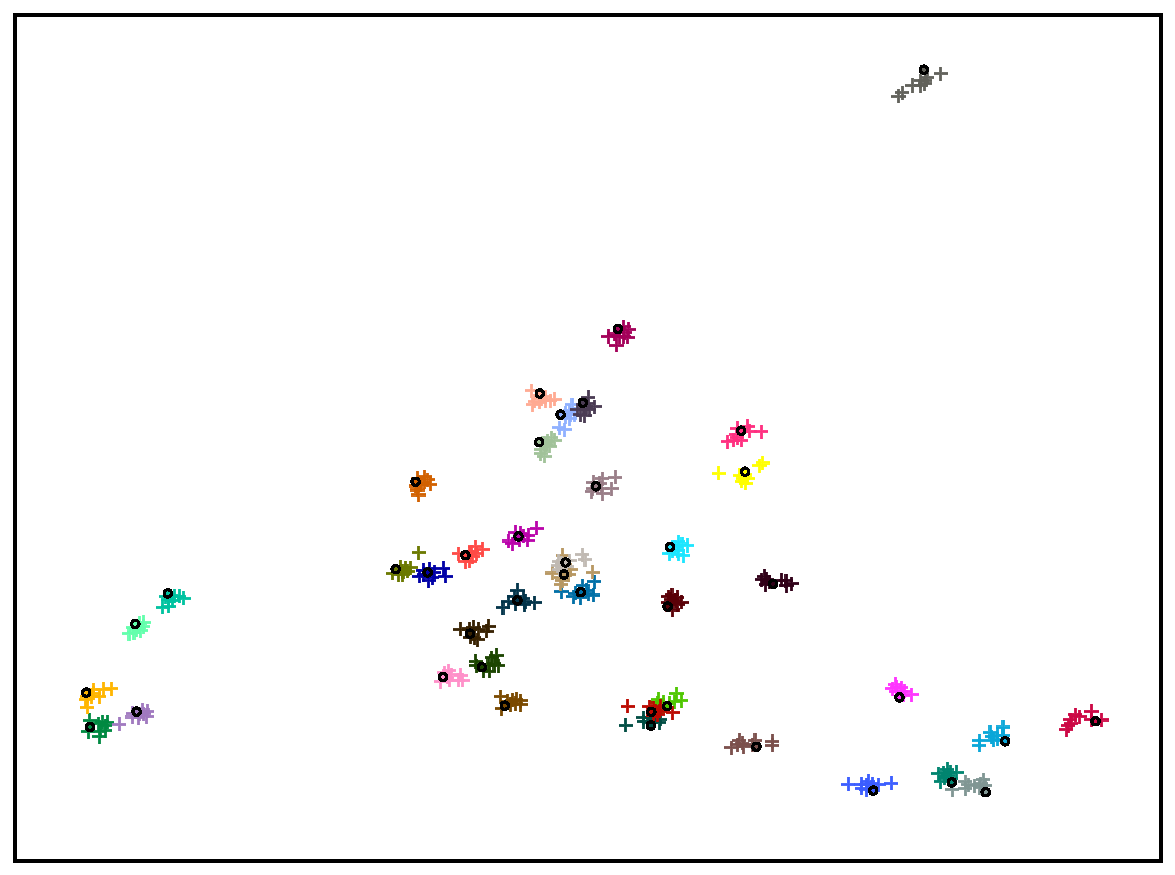
\includegraphics[width=0.95\textwidth]{graphics/MDS_Synthetic.pdf}
    \end{figure}

    \column{0.25\textwidth}
    \textsc{K-Clust} \\
    $k = 5$ \\
    $id = 0.85$ \\
    \hfill \\
    \hfill \\
    clusters: 40 \\
    max. size: 10 \\
    avg. size: 10 \\
    singletons: 0
  \end{columns}
\end{frame}

%\begin{frame}
%  \begin{figure}[h]
%    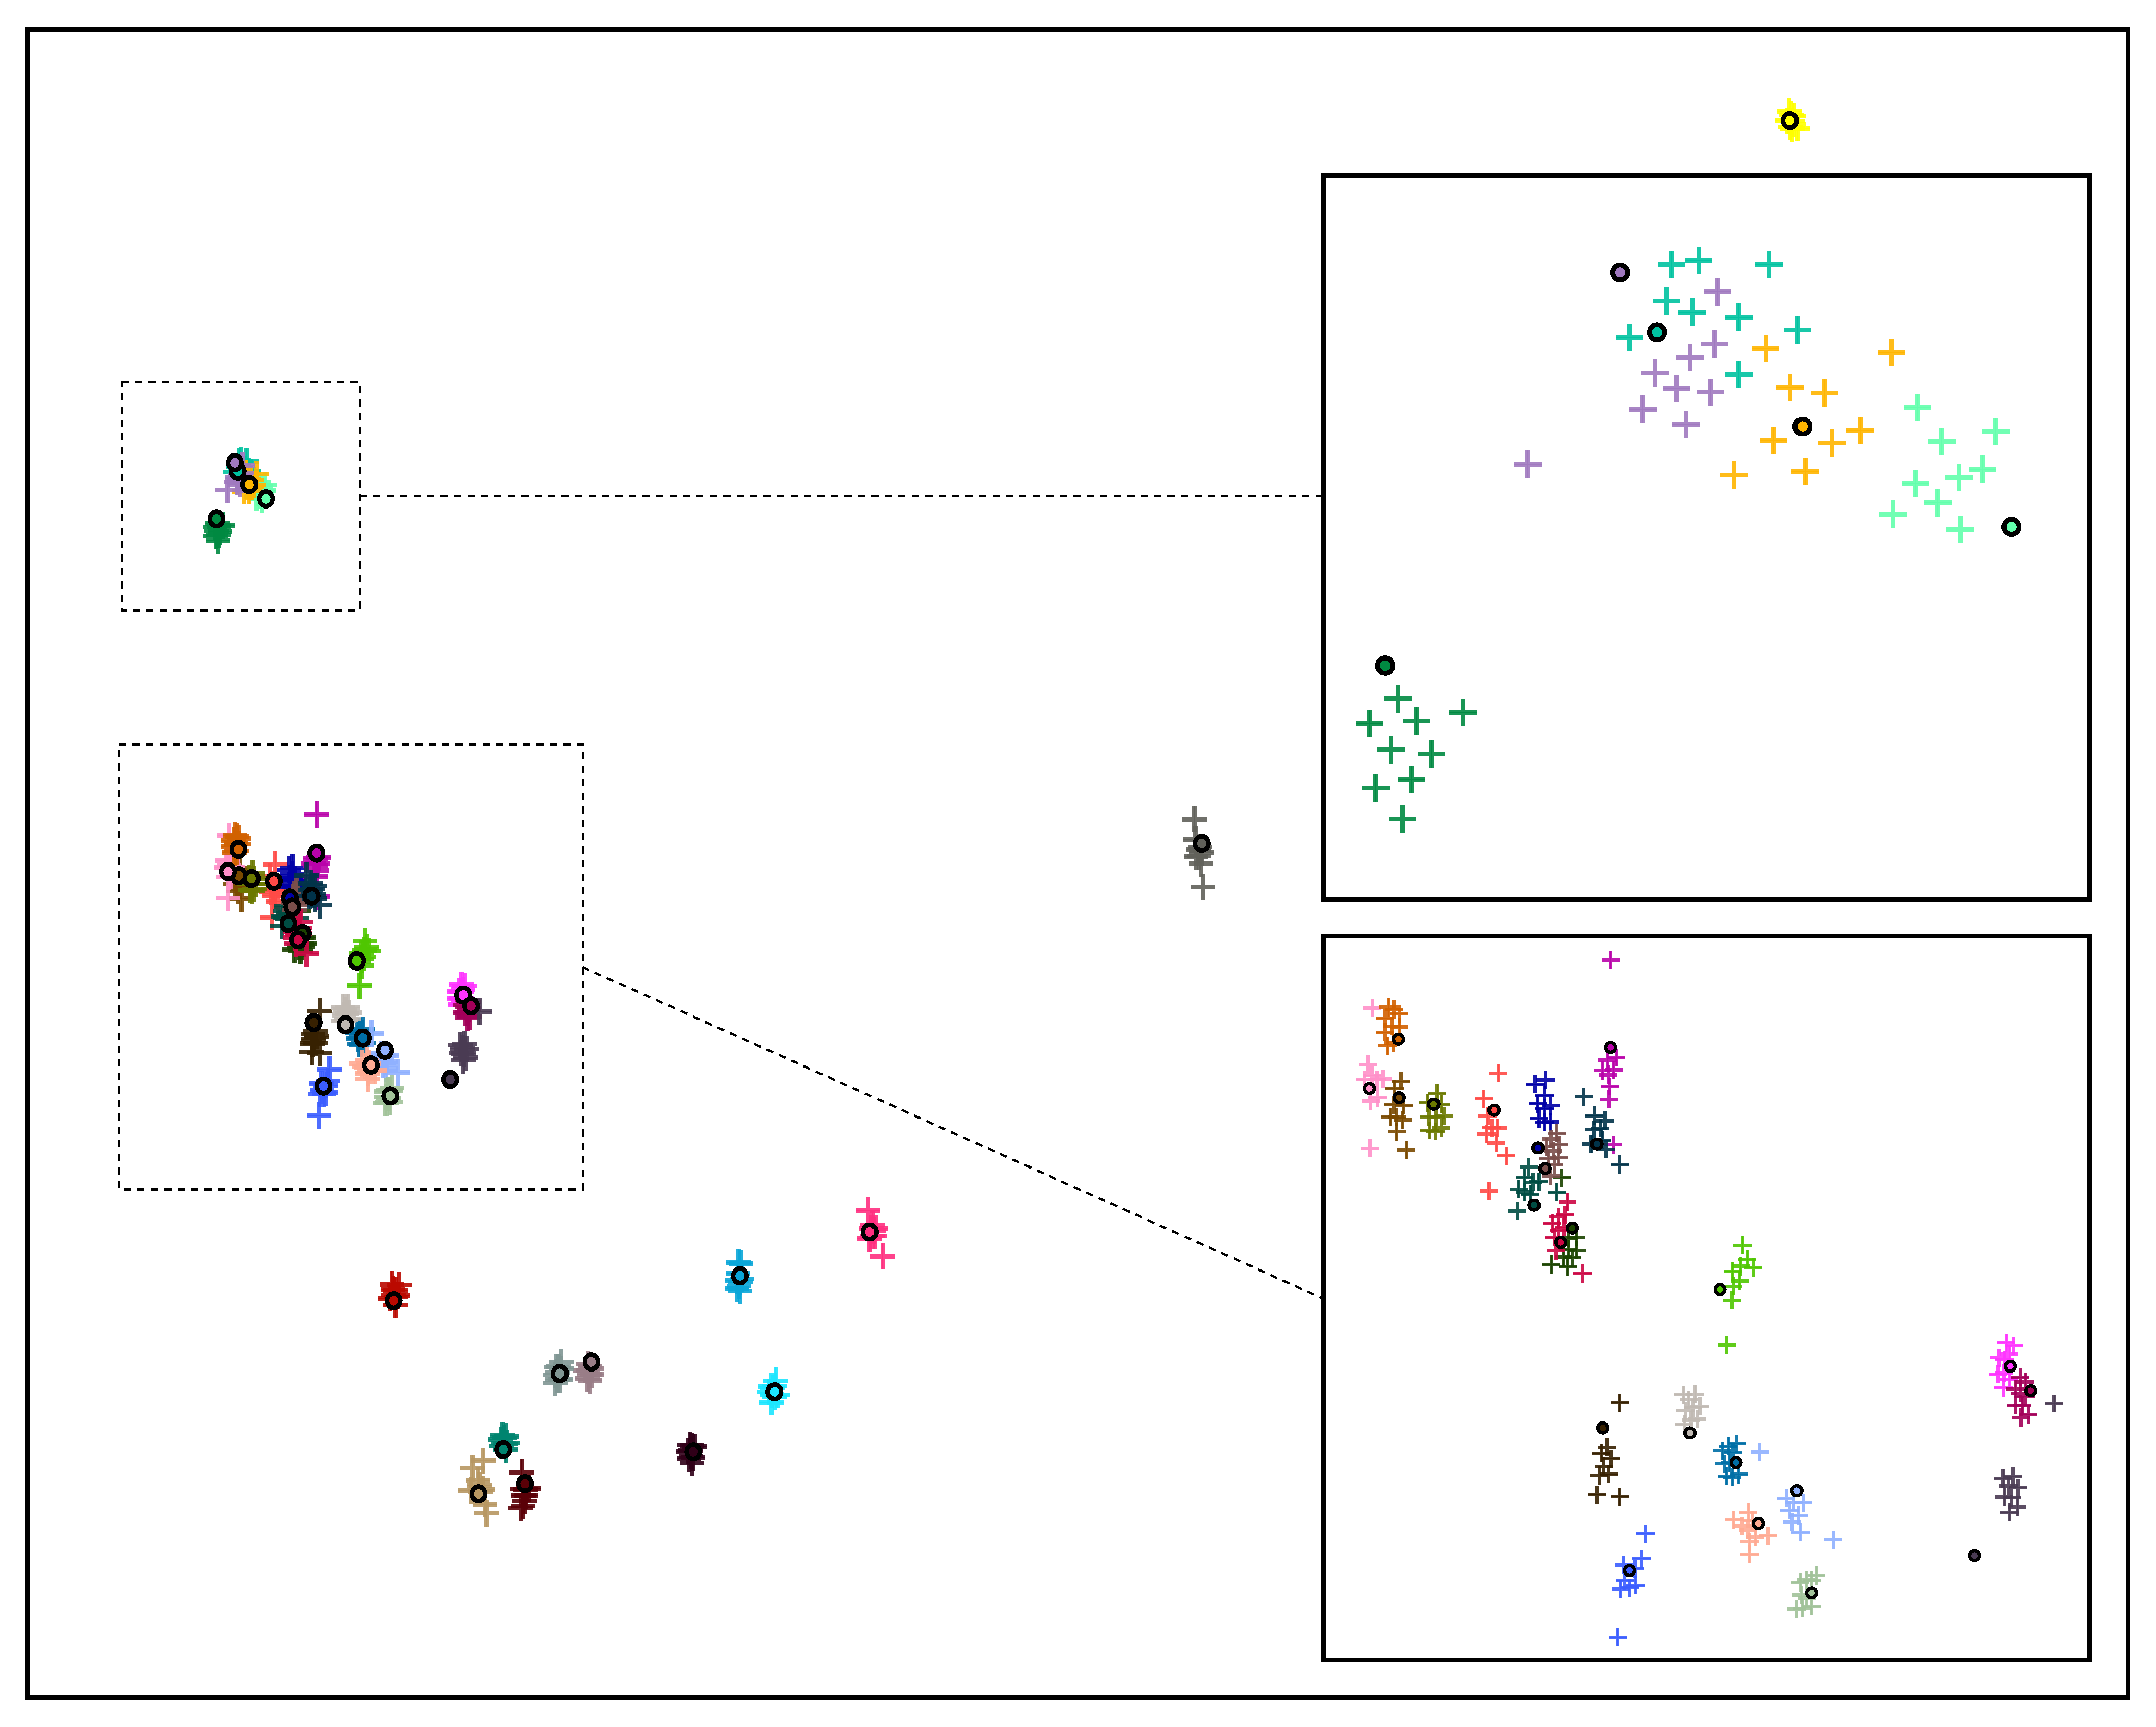
\includegraphics[width=0.9\textwidth]{graphics/MDS_Levenshtein.pdf}
%  \end{figure}
%\end{frame}

\subsection{\textsc{K-Clust} on real data (\texttt{SILVA})}

\begin{frame}
  \begin{columns}[c]
    \column{0.9\textwidth}
    \begin{figure}[h]
      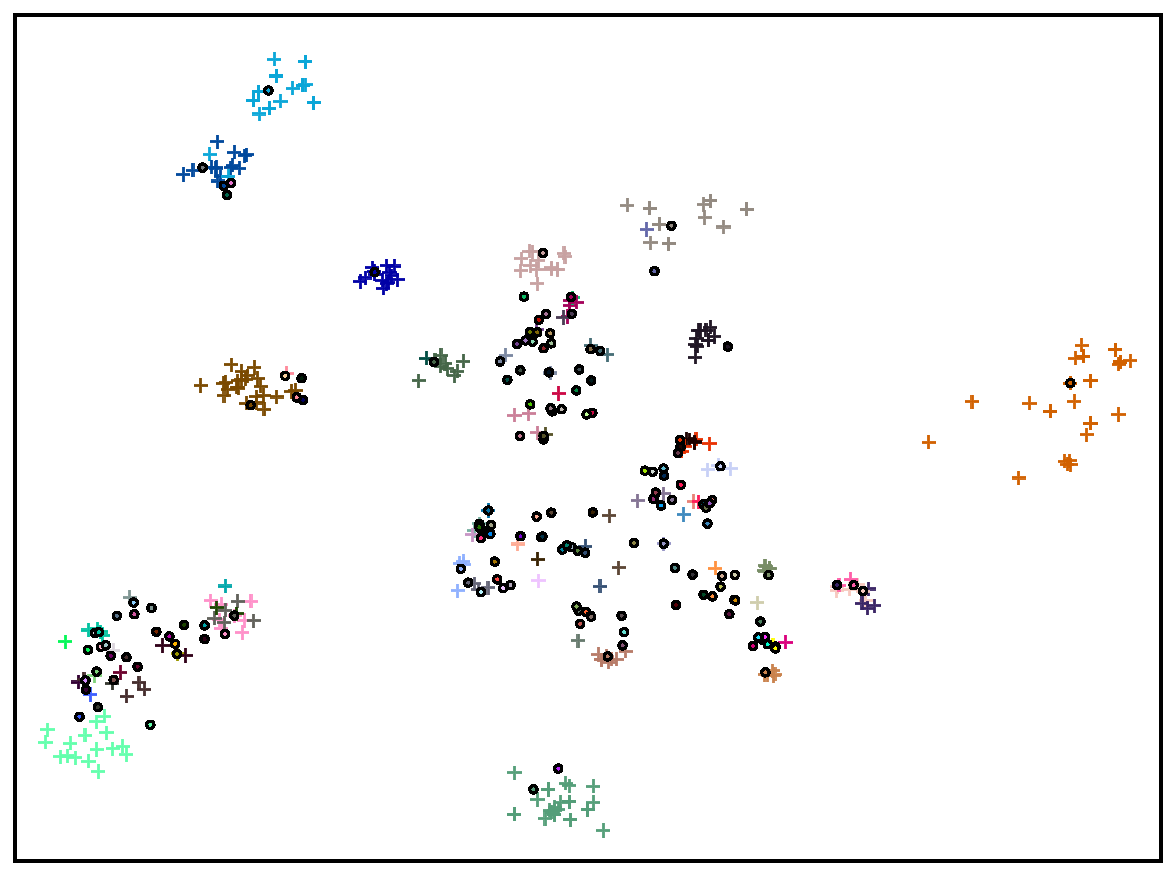
\includegraphics[width=0.95\textwidth]{graphics/MDS_Silva_incr.pdf}
    \end{figure}

    \column{0.25\textwidth}
    \textsc{K-Clust} \\
    $k = 5$ \\
    $id = 0.85$ \\
    sort: incr. \\
    \hfill \\
    clusters: 157 \\
    max. size: 43 \\
    avg. size: 3.18 \\
    singletons: 89
  \end{columns}
\end{frame}
% }}}

\end{document}
